\section{Beweis für die Existenz}
%%%%% Magnetisches Feld %%%%%
%% #1 Beweis für die Existenz %%


%Some sample text to be displayed above the first subsection

%\subsection{Prinzip}

%Ein Zyklotron besteht aus Zwei hohlen, halbzylindrischen und Duanden an denen eine Spannung mit unterschiedlichem Vorzeichen anliegt, und darüber bzw. darunter liegende Magneten, die ein homogenes Magnetfeld erzeugen. Zudem gibt es einen Einlass und einen Auslass für Teilchen.

%\begin{wrapfigure}{r}{0.4\textwidth} \label{Zyklo}
%
%	\vspace{-10pt}
%	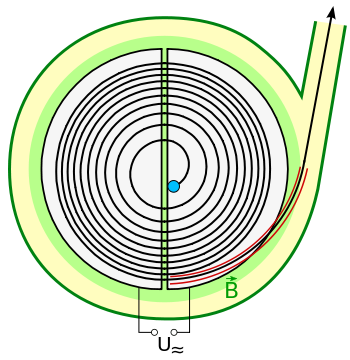
\includegraphics[width=0.35\textwidth]{Zyklotron_Prinzipskizze02.png}
%	\vspace{-13pt}
%	\caption{Prinzipskizze eines Zyklotrons}
%	\vspace{-5pt}	
%	
%\end{wrapfigure}

%\subsubsection{Anwendung}

% Some Formula:

%\begin{equation}
%	x= \frac{y \cdot 13 \pi z}
%			{\cos \alpha}
%\end{equation}

%%%%%%%%%%%%%%%%%%%%%%%
% Eigentlicher Beginn %
%%%%%%%%%%%%%%%%%%%%%%%


Man hat festgestellt, dass es noch ein weiteres Etwas mit Feldeigenschaften gibt, das Ähnlichkeiten mit dem Gravitationsfeld zeigt. Die wichtigste gemeinsame Eigenschaft ist, dass Kräfte auf bestimmte Körper ausgewirkt werden können, ohne dass ein erkennbares Medium gibt: Der magnetische Effekt ist auch im Vakuum zu beobachten. 

Diese Effekt kann durch eine Mehrzahl Ereignisse ausgelöst werden. Siehe dazu \referenz{sec:UrsachenEigenschaften}.







\section{Modellierung und Mathematisierung}
%%%%% Magnetisches Feld %%%%%
%%  %%


%Some sample text to be displayed above the first subsection

%\subsection{Prinzip}

%Ein Zyklotron besteht aus Zwei hohlen, halbzylindrischen und Duanden an denen eine Spannung mit unterschiedlichem Vorzeichen anliegt, und darüber bzw. darunter liegende Magneten, die ein homogenes Magnetfeld erzeugen. Zudem gibt es einen Einlass und einen Auslass für Teilchen.

%\begin{wrapfigure}{r}{0.4\textwidth} \label{Zyklo}
%
%	\vspace{-10pt}
%	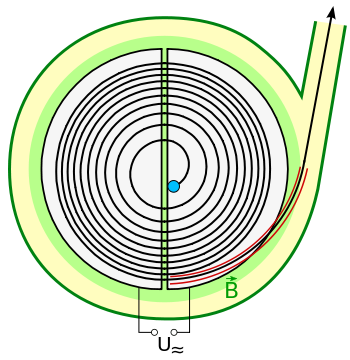
\includegraphics[width=0.35\textwidth]{Zyklotron_Prinzipskizze02.png}
%	\vspace{-13pt}
%	\caption{Prinzipskizze eines Zyklotrons}
%	\vspace{-5pt}	
%	
%\end{wrapfigure}

%\subsubsection{Anwendung}

% Some Formula:

%\begin{equation}
%	x= \frac{y \cdot 13 \pi z}
%			{\cos \alpha}
%\end{equation}

%%%%%%%%%%%%%%%%%%%%%%%
% Eigentlicher Beginn %
%%%%%%%%%%%%%%%%%%%%%%%


\subsection{Feldlinien}

Wie schon beim elektrischen Feld wird hier ein Feldlinienmodell genutzt um Eigenschaften wie Ausrichtung (Polung) oder Stärke darzustellen. 

Magnetische Felder haben 2 Pole, die nicht negativ oder positiv, wie beim elektrischen Feld, sondern Nord- und Südpol genannt werden. Ungleichnamige Pole ziehen sich an, gleichnamige stoßen sich ab. Im Feldlinienmodell zeigen die Pfeile immer zum Südpol.

Charakteristische Bilder von Feldlinien sowie Erklärungen zu diesen finden sich in \referenz{sec:feldlinienbilder}.


\subsection{Magnetische Flussdichte}

Auch beim magnetischen Feld gibt die Dichte der Feldlinien eine die Stärke des Feldes an. Diese Größe heißt aber nicht Feldstärke sondern \glqq magnetische Flussdichte \grqq{} (Formelzeichen $B$, Einheit \glqq Telsa\grqq : $T=\frac{kg}{As^2}=\frac{Vs}{m^2}$) (die magnetische Feldstärke gibt es auch, bezeichnet aber etwas anderes!). Diese ist also äquivalent zur Feldstärke des elektrischen Feldes und ordnet über die Lorentzkraft jedem bewegten, geladenen Teilchen eine Kraft zu (Siehe \referenz{subsec:BLorentzDefinition}).


\subsection{Homogenes Feld} \label{subsec:MFeldHomogen}

Ein homogenes Magnetfeld hat die Eigenschaft, dass die Flussdichte in jedem Punkt gleich ist, was Berechnungen erheblich einfacher macht. (Vergleiche: \referenz{subsec:EFeldHomogen}) Homogene Felder treten zum Beispiel im Inneren von Spulen oder zwischen den Schenkeln eines Hufeisenmagneten auf. Mehr dazu in \referenz{sec:feldlinienbilder}.




















\section{Ursachen und Eigenschaften eines Magnetfeldes} \label{sec:UrsachenEigenschaften}
%%%%% Magnetisches Feld %%%%%
%% #1 Beweis für die Existenz %%


%Some sample text to be displayed above the first subsection

%\subsection{Prinzip}

%Ein Zyklotron besteht aus Zwei hohlen, halbzylindrischen und Duanden an denen eine Spannung mit unterschiedlichem Vorzeichen anliegt, und darüber bzw. darunter liegende Magneten, die ein homogenes Magnetfeld erzeugen. Zudem gibt es einen Einlass und einen Auslass für Teilchen.

%\begin{wrapfigure}{r}{0.4\textwidth} \label{Zyklo}
%
%	\vspace{-10pt}
%	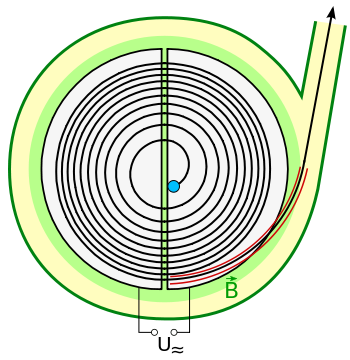
\includegraphics[width=0.35\textwidth]{Zyklotron_Prinzipskizze02.png}
%	\vspace{-13pt}
%	\caption{Prinzipskizze eines Zyklotrons}
%	\vspace{-5pt}	
%	
%\end{wrapfigure}

%\subsubsection{Anwendung}

% Some Formula:

%\begin{equation}
%	x= \frac{y \cdot 13 \pi z}
%			{\cos \alpha}
%\end{equation}

%%%%%%%%%%%%%%%%%%%%%%%
% Eigentlicher Beginn %
%%%%%%%%%%%%%%%%%%%%%%%

\subsection{Ferromagnetisches Metall}

Ein magnetisches Feld wird im klassischsten Sinne ausgelöst, wenn ein ferromagnetisches Metall \glqq magnetisiert\grqq{} wird, was heißt, dass sich sogenannte Elementarmagnete ausrichten.\footnote{Siehe: \url{https://de.wikipedia.org/wiki/Elementarmagnet}}


\subsection{Elektromagnet}

Jegliche Leiter, auch nicht-ferromagnetischer Natur, lösen ein magnetisches Feld aus, wenn Strom durch sie fließt.

Wenn Strom (also Elektronen, die kleinste Einheit der negativen Ladung) durch einen Leiter fließt, ergibt sich ein magnetisches Feld dessen Ausrichtung gemäß verschiedener Handregeln erfolgt. Siehe dazu \referenz{subsec:Faustregel}.


\subsection{Erdmagnetfeld}

Auch von der Erde geht ein magnetisches Feld aus, welches z.B. für Kompanten genutzt wird.




\section{Feldlinienbilder} \label{sec:feldlinienbilder}
%%%%% Magnetisches Feld %%%%%
%%  %%


%Some sample text to be displayed above the first subsection

%\subsection{Prinzip}

%Ein Zyklotron besteht aus Zwei hohlen, halbzylindrischen und Duanden an denen eine Spannung mit unterschiedlichem Vorzeichen anliegt, und darüber bzw. darunter liegende Magneten, die ein homogenes Magnetfeld erzeugen. Zudem gibt es einen Einlass und einen Auslass für Teilchen.

%\begin{wrapfigure}{r}{0.4\textwidth} \label{Zyklo}
%
%	\vspace{-10pt}
%	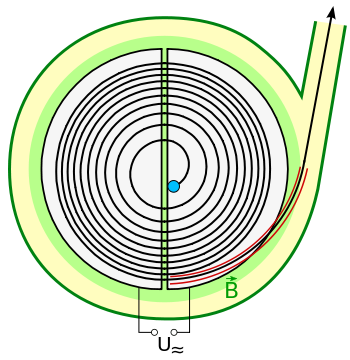
\includegraphics[width=0.35\textwidth]{Zyklotron_Prinzipskizze02.png}
%	\vspace{-13pt}
%	\caption{Prinzipskizze eines Zyklotrons}
%	\vspace{-5pt}	
%	
%\end{wrapfigure}

%\subsubsection{Anwendung}

% Some Formula:

%\begin{equation}
%	x= \frac{y \cdot 13 \pi z}
%			{\cos \alpha}
%\end{equation}

%%%%%%%%%%%%%%%%%%%%%%%
% Eigentlicher Beginn %
%%%%%%%%%%%%%%%%%%%%%%%

\subsection{Faustregel}	\label{subsec:Faustregel}

Als Eselsbrücke zur Bestimmung der Richtung der Feldlinien um den stromdurchflossenen Leiter kann die Faustregel herangezogen werden. Diese besagt, dass bei der physikalischen Stromrichtung (auch Elektronenflussrichtung genannt) die Feldlinien in Richtung der Fingerspitzen der linken Hand verlaufen, wenn der nur der Daumen abgespreizt wird und die Flussrichtung angibt.

Für die technische Stromrichtung gilt dieselbe Regel, bloß, dass mit der rechten Faust verfahren wird.

\begin{leftbar}
	Wichtig! Die physikalische Stromrichtung geht von der Bewegung der Elektronen, also der negativen Ladung aus. Diese fließen vom Minuspol zum Pluspol. Die technische Stromrichtung dagegen geht davon aus, dass die positiven Ladungen sich vom Pluspol zum Minuspol bewegen. Durch die Verwendung gespiegelter Handregeln (die jeweils andere Hand wird genommen) bleiben die Effekte jedoch dieselben. 
	
	Allgemein wird in der Physik die physikalische Stromrichtung und damit die \emph{linken} Handregeln bevorzugt, da es auch wirklich die Elektronen sind, die sich in einem Leiter bewegen.
\end{leftbar}

\subsection{Dauermagneten}  	\label{subsec:DauermagnetFeld}

%„Stromschleife“ von 30px MovGP0 - selbst erstellt mit Inkscape. Lizenziert unter CC BY-SA 2.0 de über Wikimedia Commons - https://commons.wikimedia.org/wiki/File:Stromschleife.svg#/media/File:Stromschleife.svg
%„Gerader leiter“ von Talos aus der deutschsprachigen Wikipedia. Lizenziert unter CC BY-SA 3.0 über Wikimedia Commons - https://commons.wikimedia.org/wiki/File:Gerader_leiter.svg#/media/File:Gerader_leiter.svg
%„VFPt cylindrical coil real“ von Geek3 - Eigenes WerkThis plot was created with VectorFieldPlot. Lizenziert unter CC BY-SA 3.0 über Wikimedia Commons - https://commons.wikimedia.org/wiki/File:VFPt_cylindrical_coil_real.svg#/media/File:VFPt_cylindrical_coil_real.svg
%https://lp.uni-goettingen.de/get/text/3791
%https://lp.uni-goettingen.de/get/text/3791

 \hfill

\begin{figure}[ht!]
	\centering
	\begin{minipage}[b]{0.4\linewidth}
    	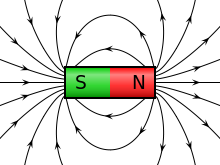
\includegraphics[width=\textwidth]{Stabmagnet}
		\caption{Das Magnetfeld um einen Stabmagnet.}
	\end{minipage}
	\quad
	\begin{minipage}[b]{0.4\linewidth}
    	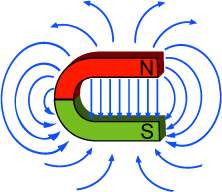
\includegraphics[width=0.6\textwidth]{Hufeisen}
		\caption{Das Magnetfeld an einem Hufeinenmagnet. Interessant ist der homogene Bereich zwischen den Schenkeln.}
	\end{minipage}
\end{figure}


\subsection{Gerader Leiter} 
\footnote{\url{https://lp.uni-goettingen.de/get/text/3791}} 
\footnote{„Gerader leiter“ von Talos aus der deutschsprachigen Wikipedia. Lizenziert unter CC BY-SA 3.0 über Wikimedia Commons - \url{https://commons.wikimedia.org/wiki/File:Gerader_leiter.svg}} 
\footnote{„Stromschleife“ von 30px MovGP0 - selbst erstellt mit Inkscape. Lizenziert unter CC BY-SA 2.0 de über Wikimedia Commons - \url{https://commons.wikimedia.org/wiki/File:Stromschleife.svg}} 
\label{subsec:GeraderLeiterFeld}

\hfill

\begin{figure}[ht!]
	\centering
	\begin{minipage}[b]{0.4\linewidth}
   	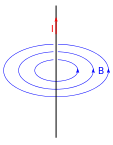
\includegraphics[width=\textwidth]{GeraderLeiter}
		\caption{Das Magnetfeld um einen geraden Leitern. $I$ zeigt die \emph{technische} Stromrichtung an.}
	\end{minipage}
	\quad
	\begin{minipage}[b]{0.4\linewidth}
    	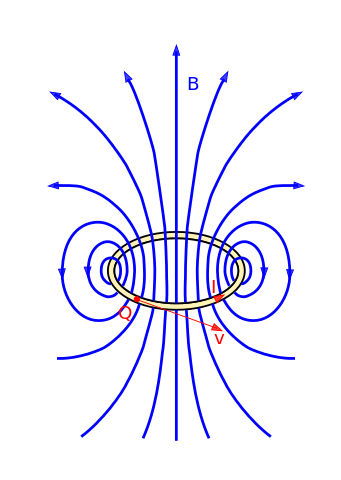
\includegraphics[width=\textwidth]{Stromschleife}
	\caption{Das Magnetfeld um eine Leiterschleife (Spule mit nur einer Windung). Man nehme Notiz von der Art, wie sich die einzelnen Feldlinien um den Leiter herum in der Mitte zu einem Bündel Feldlinien akkumulieren. $Q$ zeigt die \emph{technische} Stromrichtung an.}
	\end{minipage}
\end{figure}

\newpage
\subsection{Spule}	
\footnote{„VFPt cylindrical coil real“ von Geek3 - Eigenes WerkThis plot was created with VectorFieldPlot. Lizenziert unter CC BY-SA 3.0 über Wikimedia Commons - \url{https://commons.wikimedia.org/wiki/File:VFPt_cylindrical_coil_real.svg}}
\label{subsec:Spule}

\hfill

\begin{figure}[ht!]
	\centering
   	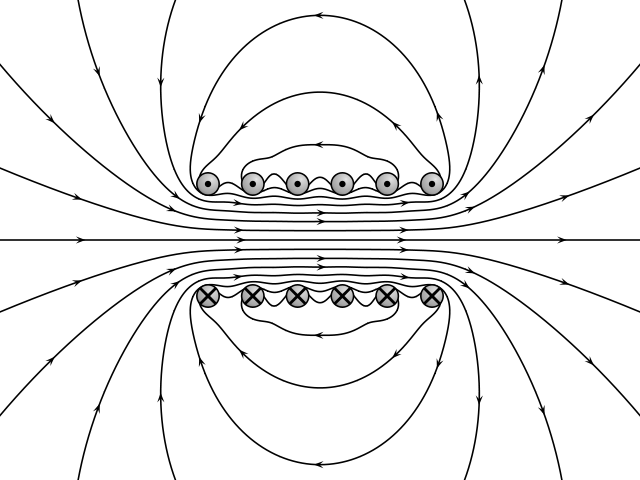
\includegraphics[width=0.8\textwidth]{Spule}
		\caption{Das Magnetfeld im Inneren einer Spule. Im Querschnitt zeigt $\otimes$ den technischen Stromfluss in die Ebene an. Vergleichbar mit der Leiterschleife, aber mit deutlich homogenerer Flussdichte im Inneren.}
\end{figure}






\section{Lorentzkraft} \label{sec:lorentzkraft}
%%%%% Magnetisches Feld %%%%%
%%  %%


%Some sample text to be displayed above the first subsection

%\subsection{Prinzip}

%Ein Zyklotron besteht aus Zwei hohlen, halbzylindrischen und Duanden an denen eine Spannung mit unterschiedlichem Vorzeichen anliegt, und darüber bzw. darunter liegende Magneten, die ein homogenes Magnetfeld erzeugen. Zudem gibt es einen Einlass und einen Auslass für Teilchen.

%\begin{wrapfigure}{r}{0.4\textwidth} \label{Zyklo}
%
%	\vspace{-10pt}
%	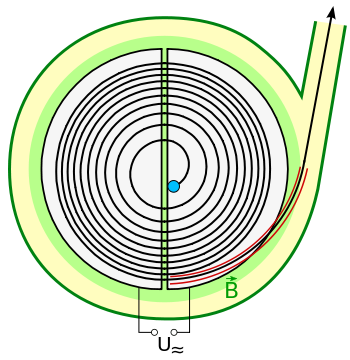
\includegraphics[width=0.35\textwidth]{Zyklotron_Prinzipskizze02.png}
%	\vspace{-13pt}
%	\caption{Prinzipskizze eines Zyklotrons}
%	\vspace{-5pt}	
%	
%\end{wrapfigure}

%\subsubsection{Anwendung}

% Some Formula:

%\begin{equation}
%	x= \frac{y \cdot 13 \pi z}
%			{\cos \alpha}
%\end{equation}

%%%%%%%%%%%%%%%%%%%%%%%
% Eigentlicher Beginn %
%%%%%%%%%%%%%%%%%%%%%%%

\subsection{Geladenes Teilchen}

Die Lorentzkraft wirkt auf jedes geladenes, in einem Magnetfeld bewegtes Teilchen, wenn sich dieses Teilchen nicht parallel zu den Feldlinien bewegt. Die Lorentzkraft ist abhängig von der Flussdichte des Magnetfeldes, der Ladung und Geschwindigkeit des Teilchens und von dem Winkel zu den Feldlinien. Im Folgenden werden jedoch nur noch Fälle betrachtet, bei denen sich Teilchen senkrecht zu den Feldlinien bewegen.


\subsection{Stromdurchflossener Leiter}

Durch einen stromdurchflossenen Leiter fließen Elektronen vom Minuspol zum Pluspol. Da Elektronen negativ geladene Teilchen sind, wirkt auch in diesem Fall die Lorentzkraft, wenn sich der Leiter in einem magnetischen Feld befindet.


\subsection{Handregeln}

\begin{figure}[h!]
	\centering
	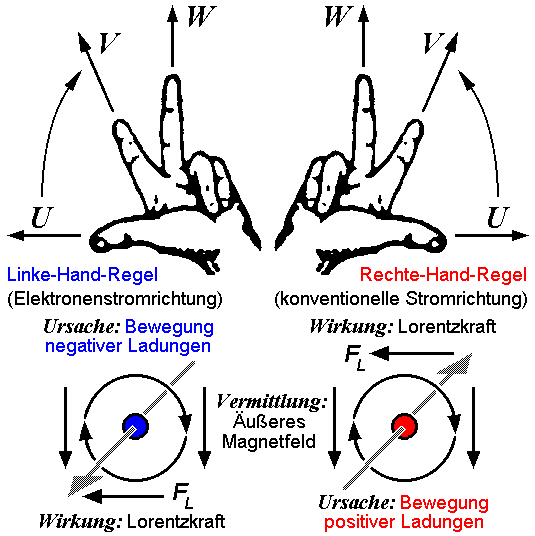
\includegraphics[width=0.65\textwidth]{Handregeln}
	\caption{Die beiden Handregeln für negative und die positive Teilchen. Die Linke gilt zudem für die physikalische und die Rechte für die Technische Stromrichtung. U: Ursache, V: Vermittlung, W: Wirkung}
	\label{fig:Handregeln}
\end{figure}

Bei der Richtung der Lorentzkraft auf ein negativ geladenes Teilchen, dass sich senkrecht zu den Feldlinien eines magnetischen Feldes bewegt, gilt die linke Handregel. Bei dieser werden Daumen, Zeige- und Mittelfinger der linken Hand abgespreizt, sodass sie der Zeichnung \referenz{fig:Handregeln}\footnote{„UVWREGEL new“ von UVWREGEL.png: Qniemiec 19:15, 14. Jan. 2011 (CET).Original uploader was Qniemiec at de.wikipediaderivative work: Qniemiec (talk) - UVWREGEL.png. Lizenziert unter CC BY-SA 3.0 über Wikimedia Commons - \url{https://commons.wikimedia.org/wiki/File:UVWREGEL\_new.png}} entsprechen. Dann bezeichnet der Daumen die Richtung des Teilchen, der Zeigefinger folgt der Richtung des Magnetfeldes und der Mittelfinder zeigt die Richtung der Lorentzkraft an. Für die Kraft auf einen Leiter der senkrecht in einem Magnetfeld steht, gilt dieselbe Regel und der Daumen zeigt die physikalische Stromrichtung an.

Für ein positives Teilchen oder die technische Stromrichtung kommt die rechte Hand zum Einsatz; die Regel für die Bezeichnung der Finger bleibt gleich.


\subsection{Gleichung} \label{subsec:BLorentzDefinition}

Der Betrag der Lorentzkraft lässt sich wie folgt berechnen:

\begin{align} \label{eq:Lorentzkraft}
\begin{split}
	F_{Lr} = q \cdot B \cdot v
\end{split}
\end{align}

\noindent Interessant ist, dass die Lorentzkraft nicht nur von der Ladung, sondern auch von der Geschwindigkeit abhängig ist. Dies macht man sich z.B. im Massenspektrometer (Siehe: \referenz{sec:Massenspektrometer}) oder im Wien'schen Filter (Siehe: \referenz{sec:Wien}) zu Nutze.

Aus der Lorentzkraft lässt sich auch die Flussdichte $B$ definieren: Die Flussdichte ordnet jedem bewegten, geladenen Körper eine Kraft (die Lorentzkraft) zu:

\begin{align} \label{eq:Flussdichte}
\begin{split}
	\vec{B} = \frac{\vec{F}_{Lr}}{q \cdot \vec{v}}
\end{split}
\end{align}









\section[Fadenstrahlrohr]{Spezifische Ladung und Elektronenmasse per Fadenstrahlrohr} \label{sec:Fadenstrahlrohr}
%%%%% Magnetisches Feld %%%%%
%%  %%


%Some sample text to be displayed above the first subsection

%\subsection{Prinzip}

%Ein Zyklotron besteht aus Zwei hohlen, halbzylindrischen und Duanden an denen eine Spannung mit unterschiedlichem Vorzeichen anliegt, und darüber bzw. darunter liegende Magneten, die ein homogenes Magnetfeld erzeugen. Zudem gibt es einen Einlass und einen Auslass für Teilchen.

%\begin{wrapfigure}{r}{0.4\textwidth} \label{Zyklo}
%
%	\vspace{-10pt}
%	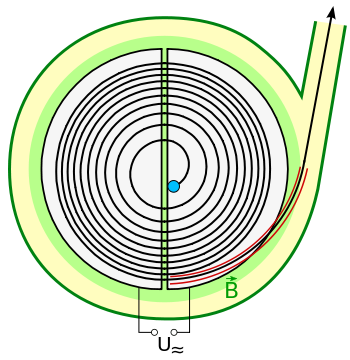
\includegraphics[width=0.35\textwidth]{Zyklotron_Prinzipskizze02.png}
%	\vspace{-13pt}
%	\caption{Prinzipskizze eines Zyklotrons}
%	\vspace{-5pt}	
%	
%\end{wrapfigure}

%\subsubsection{Anwendung}

% Some Formula:

%\begin{equation}
%	x= \frac{y \cdot 13 \pi z}
%			{\cos \alpha}
%\end{equation}

%%%%%%%%%%%%%%%%%%%%%%%
% Eigentlicher Beginn %
%%%%%%%%%%%%%%%%%%%%%%%

Das Fadenstrahlrohr illustriert die Lorentzkraft und diente zur Bestimmung der spezifischen Elektronenladung ($\frac{e}{m_e}$). Zusammen mit den Ergebnissen des Millikanversuchs (siehe: \referenz{sec:Millikan}) kann sogar die Masse eines Elektron bestimmt werden.

\subsection{Aufbau}

Ein Fadenstrahlrohr besteht aus einem Glaskolben in dem sich ein Gas befindet, dass beim Kontakt mit Elektronen zum Leuchten angeregt wird. Siehe Figure \ref{fig:Fadenstrahlrohr}\footnote{„Cyclotron motion wider view“ von Marcin Białek - Eigenes Werk. Lizenziert unter GFDL über Wikimedia Commons - \url{https://commons.wikimedia.org/wiki/File:Cyclotron\_motion\_wider\_view.jpg}}

Im Inneren befindet sich zudem eine Elektronenkanone, die beschleunigte Elektronen, wie schon in der Beschreibung der Braun'schen Röhre (Siehe: \referenz{sec:BraunscheRoehre}), absondert. Durch ein Helmholzspulenpaar (2 kurze Spulen mit großem Radius) die parallel zur Richtung der beschleunigten Elektronen stehen, wird ein homogenes Magnetfeld erreicht, welches senkrecht auf der Elektronenrichtung steht.

\begin{figure}[h!]
	\centering
	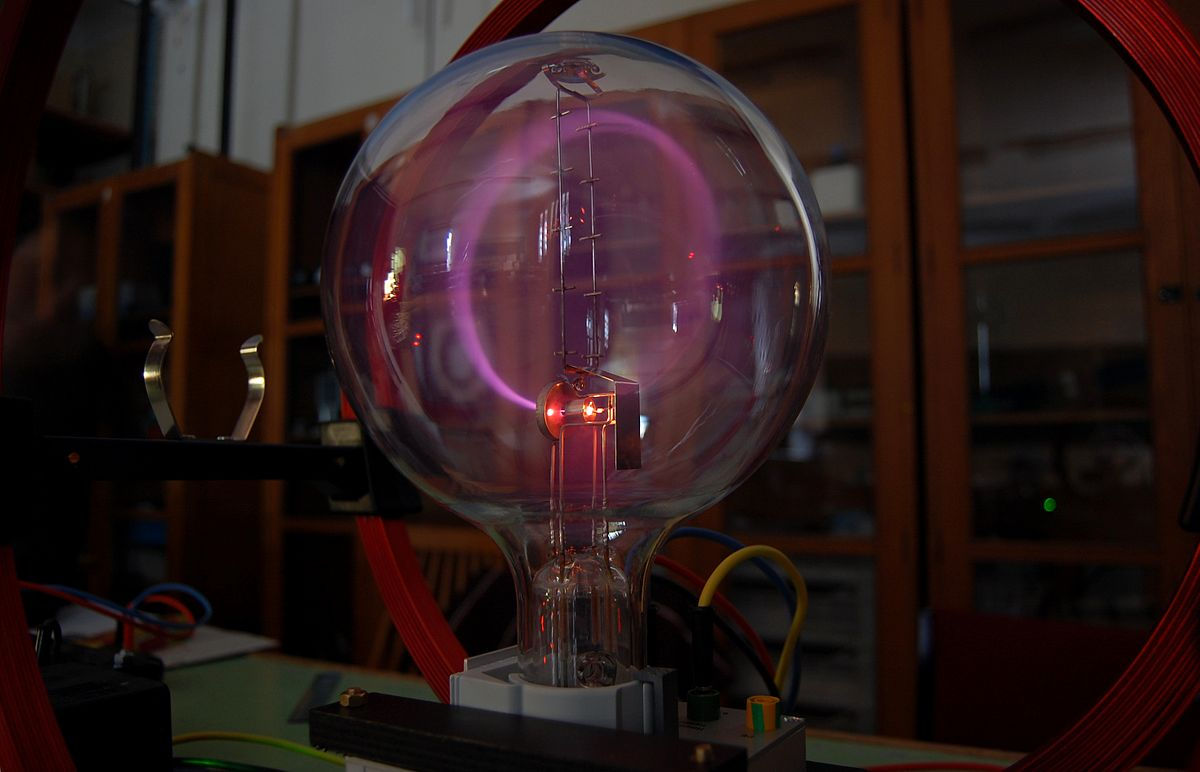
\includegraphics[width=0.8\textwidth]{Fadenstrahlrohr}
	\caption{Ein Fadenstrahlrohr}
	\label{fig:Fadenstrahlrohr}
\end{figure}

\subsection{Beobachtung}

Die Elektronen beschreiben eine Kreisbahn, was am leuchtenden Gas zu sehen ist. Damit ist die Existenz einer Kraft auf bewegte Teilchen im Magnetfeld illustriert.

\subsection{Mathematisierung}

Wenn die Geschwindigkeit der Elektronen bekannt, bzw. errechnet wurde, kann über den Radius, welcher auch gemessen werden kann, die spezifische Elektronenladung bestimmt werden. Der Ansatz ist das Gleichsetzten der allgemeinen Zentripetalkraft $F_{Zp} = m \cdot \frac{v^2}{r}$, also die Kraft, die das Elektron nach innen zieht mit der Lorentzkraft  $F_{Lr} = q \cdot B \cdot v$, welche ja genau diese Bahn bewirkt:

\begin{align}
\begin{split}
	F_{Zp} &= F_{Lr} \\
	m_e \cdot \frac{v^2}{r} &= e \cdot B \cdot v \\
	\frac{e}{m_e} &=\frac{v}{B \cdot r}
\end{split}
\end{align}

\noindent Da es 2 Variablen in der Gleichung gibt, kann man mit diesem Versuch nur auf das Verhältnis der Ladung und Masse schließen, die \glqq spezifische Elektronenmasse\grqq .

Über den Millikanversuch (siehe: \referenz{sec:Millikan}) konnte jedoch die Elektronenladung direkt bestimmt werden, sodass durch den Versuch mit dem Fadenstrahlrohr die Masse bestimmt werden konnte:

\begin{align}
\begin{split}
	\frac{e}{m_e} &=\frac{v}{B \cdot r} \\
	m_e &=\frac{e \cdot B \cdot r}{v}
\end{split}
\end{align}








\section{Wien'scher Geschwindigkeitsfilter} \label{sec:Wien}
%%%%% Magnetisches Feld %%%%%
%% Wien'sche Geschwindugkeitsfilter %%


%Some sample text to be displayed above the first subsection

%\subsection{Prinzip}

%Ein Zyklotron besteht aus Zwei hohlen, halbzylindrischen und Duanden an denen eine Spannung mit unterschiedlichem Vorzeichen anliegt, und darüber bzw. darunter liegende Magneten, die ein homogenes Magnetfeld erzeugen. Zudem gibt es einen Einlass und einen Auslass für Teilchen.

%\begin{wrapfigure}{r}{0.4\textwidth} \label{Zyklo}
%
%	\vspace{-10pt}
%	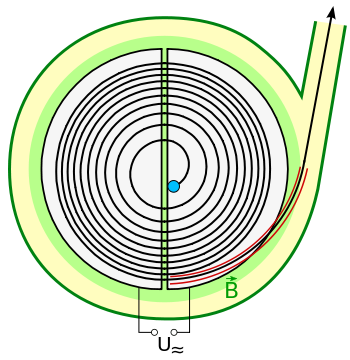
\includegraphics[width=0.35\textwidth]{Zyklotron_Prinzipskizze02.png}
%	\vspace{-13pt}
%	\caption{Prinzipskizze eines Zyklotrons}
%	\vspace{-5pt}	
%	
%\end{wrapfigure}

%\subsubsection{Anwendung}

% Some Formula:

%\begin{equation}
%	x= \frac{y \cdot 13 \pi z}
%			{\cos \alpha}
%\end{equation}

%%%%%%%%%%%%%%%%%%%%%%%
% Eigentlicher Beginn %
%%%%%%%%%%%%%%%%%%%%%%%

Der Wien'sche Geschwindigkeitsfilter ist eine Möglichkeit, einen Elektronenstrahl nach seiner Geschwindigkeit zu filtern, das heißt nur Elektronen mit einer gewissen Geschwindigkeit passieren zu lassen.

\subsection{Aufbau}

\begin{figure}[h!]
	\centering
	\vspace*{-10pt}
	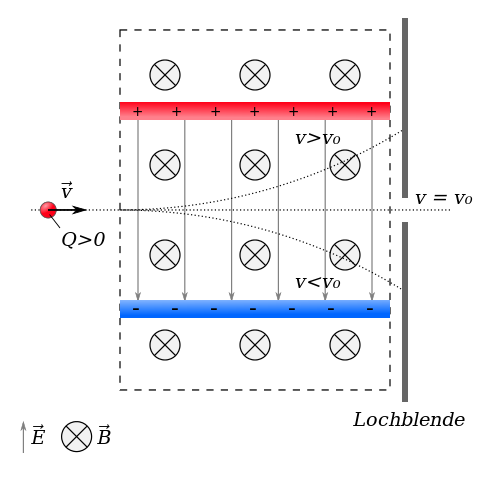
\includegraphics[width=0.6\textwidth]{Wien}
	\caption{Der Geschwindigkeitsfilter nach Wien}
	\label{fig:Wien}
\end{figure}

Grundbaustein bildet eine Ablenkeinheit mit einem Kondensator, wie sie in der Braun'schen Röhre (Siehe: \referenz{sec:BraunscheRoehre}) verwendet wird. Allerdings wird nun ein homogenes Magnetfeld so über den Kondensator gelegt, dass die Feldlinien dieses Feldes senkrecht auf der Elektronenrichtung \emph{und} der Feldlinien des elektrischen Feldes stehen.

Abbildung \ref{fig:Wien} \footnote{„Geschwindigkeitsfilter nach Wien“ von Miessen - Eigenes Werk. Lizenziert unter CC0 über Wikimedia Commons - \url{https://commons.wikimedia.org/wiki/File:Geschwindigkeitsfilter\_nach\_Wien.svg}} zeigt den schematischen Aufbau, jedoch werden positiv geladene Körper ($Q>0$) betrachtet und nicht wie hier Elektronen.


\begin{leftbar}
	Anmerkung: Da die magnetischen Feldlinien nicht zeichenbar sind, da sie \glqq in die Papierebene\grqq{} gehen. Dafür wird $\odot$ verwendet, um Anzuzeigen, dass der Pfeil aus der Ebene hinaus verläuft und $\otimes$ um Anzuzeigen, dass der Pfeil in die Ebene hinein verläuft.
	
	Eselsbrücke: Wenn man mit einem Bogen einen Pfeil verschießt, sie man das Kreuz der Federn; im letzten Moment, bevor man von einem getroffen wird, sieht man den Punkt der Pfeilspitze.
\end{leftbar}



\subsection{Funktionsweise}

Das Magnetfeld und der Kondensator werden so gepolt, dass die, gemäß linker Handregel resultierende, Lorentzkraft $F_{Lr}$ der Coulombkraft $F_{el}$ entgegenwirkt. Da die Lorentzkraft abhängig von der Geschwindigkeit des Teilchens ist und die elektrische Kraft nicht, ergibt sich eine Geschwindigkeit bei der sich die beiden Kräft die Waage halten:

\begin{align}
\begin{split}
	F_{Lr} &= F_{el} \\
	e \cdot B \cdot v &= e \cdot E \\
	v &= \frac{E}{B}
\end{split}
\end{align}

\noindent \emph{Man nehme Notiz von dieser simplen und unglaublich schönen Beziehung!}

Eine Einheitenrechung folgt:

\begin{align}
\begin{split}
	v &= \frac{E}{B} \\
	\frac{m}{s} &= \frac{N}{C} \cdot \frac{1}{T} \\
	\frac{m}{s} &= \frac{kg \cdot m}{s^2 \cdot As} \cdot \frac{As^2}{kg} \\
	\frac{m}{s} &= \frac{m}{s}
\end{split}
\end{align}





















\section{Massenspektrometer} \label{sec:Massenspektrometer}
%%%%% Magnetisches Feld %%%%%
%% Massenspektrometer %%


%Some sample text to be displayed above the first subsection

%\subsection{Prinzip}

%Ein Zyklotron besteht aus Zwei hohlen, halbzylindrischen und Duanden an denen eine Spannung mit unterschiedlichem Vorzeichen anliegt, und darüber bzw. darunter liegende Magneten, die ein homogenes Magnetfeld erzeugen. Zudem gibt es einen Einlass und einen Auslass für Teilchen.

%\begin{wrapfigure}{r}{0.4\textwidth} \label{Zyklo}
%
%	\vspace{-10pt}
%	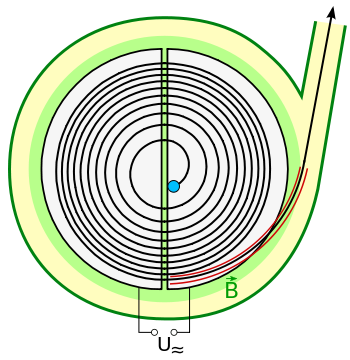
\includegraphics[width=0.35\textwidth]{Zyklotron_Prinzipskizze02.png}
%	\vspace{-13pt}
%	\caption{Prinzipskizze eines Zyklotrons}
%	\vspace{-5pt}	
%	
%\end{wrapfigure}

%\subsubsection{Anwendung}

% Some Formula:

%\begin{equation}
%	x= \frac{y \cdot 13 \pi z}
%			{\cos \alpha}
%\end{equation}

%%%%%%%%%%%%%%%%%%%%%%%
% Eigentlicher Beginn %
%%%%%%%%%%%%%%%%%%%%%%%

Das Massenspektrometer macht man sich zur Identifikation von chemischen Elementen und deren Isotopen die unterschiedlichen Atommassen zu Nutze. Die ersten funktionstüchtigen Massenspektrometer gibt es seit dem frühen 20. Jahrhundert.

\subsection{Aufbau}

In der Ionenquelle werden Atome aus der Probe gelöst und ionisiert. Das heißt, sie sind nun im gasförmigen Zustand und zudem positiv geladen.

Nach einer Beschleunigungseinheit und einem Wien'schen Filter werden sie in ein homogenes Magnetfeld geleitet in welchem sie dann, gemäß der Lorentzkraft auf eine Kreisbahn gezwungen werden. 

Da man absolute Gewissheit über Ladung, Geschwindigkeit hat und auch die Flussdichte des Magnetfeldes kennt, ist die einzige Variable, die den Auftreffpunkt auf der Indikatorplatte bestimmt, die Masse des Atoms. Wie beim Fadenstrahlrohr (Siehe \referenz{sec:Fadenstrahlrohr}) wird der Ansatz $F_{Zp} = F_{Lr}$ vollzogen:

\begin{align}
\begin{split}
	F_{Zp} 				  &= F_{Lr} \\
	m \cdot \frac{v^2}{r} &= q \cdot B \cdot v \\
	m 					  &= \frac{q \cdot B \cdot r}{v}
\end{split}
\end{align}













\section{Zyklotron}
%%%%% Magnetisches Feld %%%%%
%%  %%


%Some sample text to be displayed above the first subsection

%\subsection{Prinzip}

%Ein Zyklotron besteht aus Zwei hohlen, halbzylindrischen und Duanden an denen eine Spannung mit unterschiedlichem Vorzeichen anliegt, und darüber bzw. darunter liegende Magneten, die ein homogenes Magnetfeld erzeugen. Zudem gibt es einen Einlass und einen Auslass für Teilchen.

%\begin{wrapfigure}{r}{0.4\textwidth} \label{Zyklo}
%
%	\vspace{-10pt}
%	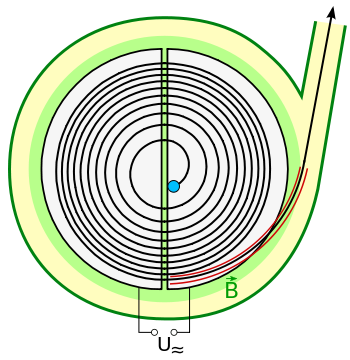
\includegraphics[width=0.35\textwidth]{Zyklotron_Prinzipskizze02.png}
%	\vspace{-13pt}
%	\caption{Prinzipskizze eines Zyklotrons}
%	\vspace{-5pt}	
%	
%\end{wrapfigure}

%\subsubsection{Anwendung}

% Some Formula:

%\begin{equation}
%	x= \frac{y \cdot 13 \pi z}
%			{\cos \alpha}
%\end{equation}

%%%%%%%%%%%%%%%%%%%%%%%
% Eigentlicher Beginn %
%%%%%%%%%%%%%%%%%%%%%%%

\subsection{Prinzip} 

Ein Zyklotron besteht aus 2 hohlen, halbzylindrischen Duanden, an denen eine Spannung mit unterschiedlichem Vorzeichen anliegt. Zwischen den Duanden befindet sich ein kleiner Zwischenraum, in welchem dann ein homogenes elektrisches Feld entsteht, dessen Feldlinien von der einen zur anderen Duande verlaufen (Siehe \referenz{subsec:EFeldHomogen}). Aus 2 darüber bzw. darunter liegenden Magneten ergibt sich ein homogenes Magnetfeld (Siehe \referenz{subsec:MFeldHomogen}).

Darüber hinaus gibt es einen Einlass und einen Auslass für Teilchen.\footnote{„Zyklotron Prinzipskizze02“ von KlausFoehl - Eigenes Werk. Lizenziert unter Gemeinfrei über Wikimedia Commons - \url{https://commons.wikimedia.org/wiki/File:Zyklotron_Prinzipskizze02.svg}}


\begin{wrapfigure}{o}{0.4\textwidth} \label{Zyklo}

	\vspace{-10pt}
	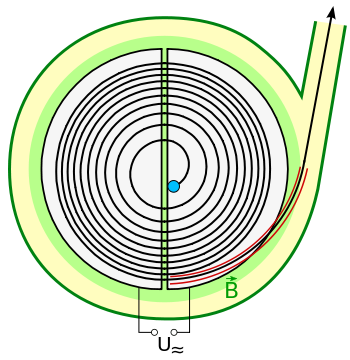
\includegraphics[width=0.35\textwidth]{Zyklotron_Prinzipskizze02.png}
	\vspace{-13pt}
	\caption{Prinzipskizze eines Zyklotrons}
	\vspace{-5pt}	
	
\end{wrapfigure}

Die Teilchenquelle im Inneren des Zyklotrons setzt Elektronen oder Protonen frei, welche durch den Einlass in das elektrische Feld zwischen den Duanden eintreten und durch dieses Feld zu einer der Beiden hin beschleunigt werden. Diese Teilchen werden gleichzeitig durch das Magnetfeld, über die Lorentzkraft, auf eine Kreisbahn gezwungen (Siehe \referenz{sec:lorentzkraft}), sodass sie im hohlen Duanden eine 180\degree{} Kurve beschreiben. Sobald wieder der Spalt zwischen den Duanden erreicht ist, wird die Spannung umgepolt, sodass die Teilchen nun zum anderen Duanden hingezogen werden. Diese Umpolungsfrequenz bleibt über den ganzen Versuch konstant.

In dem Spalt werden die Teilchen abermals und abermals beschleunigt bis der Radius so groß ist, dass die Teilchen aus dem Zyklotron austreten.


\subsection{Gesetze}

Für die Beschleunigung für \emph{Elektronen} gelten folgende Gesetzmäßigkeiten.

\subsubsection{Radius}

Aus der Gleichsetzung der Zentrifugalkraft und der Lorentzkraft ergibt sich: 

\begin{align}
\begin{split}
	F_{Zf} &= F_{Lr} \\
	\frac{m \cdot v^2}{r} &= q_e \cdot v \cdot B
\end{split}
\end{align}

\noindent Daher gilt für den Radius:

\begin{align} \label{eq:ZyklotronRadius}
\begin{split}
	r = \frac{m_e \cdot v}{B \cdot q_e}
\end{split}
\end{align}


\subsubsection{Frequenz}

Aus den Betrachtungen der Umlaufzeit $T = \frac{s_{Umlauf}}{v} = \frac{2 \pi r}{v}$ und des Radius (Siehe Gleichung \ref{eq:ZyklotronRadius}) ergibt sich für die Frequenz der Umpolung mit $f=\frac{1}{T}$: \\

\begin{align}
\begin{split}
	f &= \frac{1}{T} \\
	f &= \frac{v}{2 \pi r} \\
	f &= \frac{v \cdot q_e \cdot B}{2 \pi \cdot m_e \cdot v} \\
	f &= \frac{q_e \cdot B}{2 \pi \cdot m_e}
\end{split}
\end{align}

\noindent Damit ist gezeigt, dass die Frequenz nicht abhängig von der Geschwindigkeit der Teilchen ist und auch sonst nur von konstanten Größen abhängig ist. Daher ist die Frequenz ebenfalls über den gesamten Versuch konstant.




